\section{Overview}
% gps required
%TODO devo essere più preciso nella spiegazione delle funzioni dei vari componenti?
%TODO aggiungere anche il numero di tier e qualcosa di più specifico sulla parte hardware?
The distributed application is composed by a server side, and a client one.
The client side interacts with users (or guests), showing the correct activity, and sends requests to the server side, when needed.
The client side must be able to interact with the GPS.
The server side manages requests coming from the client side, and notifies the users (or the guests) involved in the requests.
The server side must also interact with a map system, in order to retrieve information about the route and the length of the ride.

\section{High level components and their interaction}
% aggiungere l'UML che ho fatto per il RASD? Sì da bravo
%TODO: fare un parallelo con MVC, per chiarificare le cose <---@luca: <personalmente preferirei anch'io farlo qua, ma essendoci una
								%   sessione dedicata ai pattern usati, forse è meglio inserirlo lì>
The client side is composed by a set of activities composed by one or more actions and displayed through the user interface.
The client side has also an interface which manages the interaction with the server.
The server side has a controller for each connected client, that manages the requests coming from the users (or guests), 
taking data from the ride manager. It also sends messages to the clients in order to resolve the requests.
The controller interacts with the clients through a network interface.
%TODO: sequence diagram del lato server, che è interessante da mettere
\section{Component view}
	\subsection{Client}
	 \begin{itemize}
	  \item [Activity]: an activity is a set of messages and actions, that the application must display to the users.
	  No more than one activity can be displayed at the same time;
	  The default activity is the "guest home" activity. Each time the user taps a button, the application must execute
	  the related action, and select the next activity.
	  %TODO: paragone con le activity in android
	  \item [Action]: an action is something that a user can do, in order to interact with the application.
	  If an action needs some data, the userinterface must display a field, for each input needed, that allows the human
	  to provide the necessary incormations.
	  Some actions can also select the next activity that must be shown, or/and send informations to the server,
	  in order to complete their job.
	  \item [Userinterface]: is the component that directly interacts with the human.
	  It contains the activity that must be displayed, and read the components of the activity, in order to display them.
	  It also launches the actions selected by the human.
	  \item[Clientnetworkinterface]: is the component that allows the other ones to exchange messages with the server side.
	 \end{itemize}
	\subsection{Application server}
	\begin{itemize}
	 \item [Controller]: we have one controller for each client connected; initially it will be a guest controller,
	 which allows login/register. After a successful login, the guest controller will create a taxi driver/passenger controller,
	 and substitutes himself with the new controller. The controller must manage requests coming from
	 the client, taking informations from the ridesmanager, and eventually adding new objects to it.
	 In order to send and receive messages from the client, the controller communicates with a Servernetworkinterface.
	 The controller also contains a User object, that allows him to retrieves information about the specific logged user.
	 \item [Ridesmanager]: it is a singleton, that contains informations about the queues, the active rides. This corresponds 
	 to the model in the MVC pattern and it is shared by all the controllers.
	 \item [User]: is the component that contains every possible information about a logged user, taken from the database.
	 User is a part of the controller ( obviously only in case of passenger/taxi driver controller).
	 User is split in taxi driver and passenger, cause there are some differences between the two kind of user.
	 Also user is a part of the model, but it is not shared.
	 \item[Ride]: this class allows to create object, containing all information about a specific ride. 
	 As soon as a passenger makes a taxi requests, the controller creates a ride containing information recevied from the client.
	 In case of shared ride, a ride object will be created and added to the corresponding sharedride ones.
	 \item[Sharedride]: the sharedride object contains the set of the ride object, the total cost of the ride and the route.
	 When a new passenger is added to the shared ride, the controller will adjust the path, the total cost, and the cost of each
	 rides object, contained in the current sharedride.
	 \item[Servernetworkinterface]: is the component that allows the interaction with the client side. It converts messages coming from
	 the other server component, in messages readable by the Clientnetwrokinterface, and vice versa.
	\end{itemize}
	\subsection{Master view}
	(the whole master view component is singleton)
	\begin{itemize}
	  \item [CLI:] simple text based interface, receives input from stdin, sends output to stdout
	  \item [Controller:] interprets the cli commands, and invokes the relative methods on the specific server classes;
	  the outcome of the operation is returned to the cli.
	\end{itemize}
	% In teoria basta una semplice interfaccia testuale, più un controller che interpreta gli input e chiama i
	% dovuti metodi sul Server
	\subsection{Database server}
	The database server will contain all informations about users, and, for each user, the list of unsent notifications.
	The client will periodically send notification request to the server, that must query the database, send the list of notification,
	and empty the unsent notification list.
	%TODO facciamo dei backup periodici del database in un altro database posto in una zona "sicura"?
\newpage
\section{Runtime view}
	\subsection{Sequence diagrams}
\begin{figure} [h]
\centering
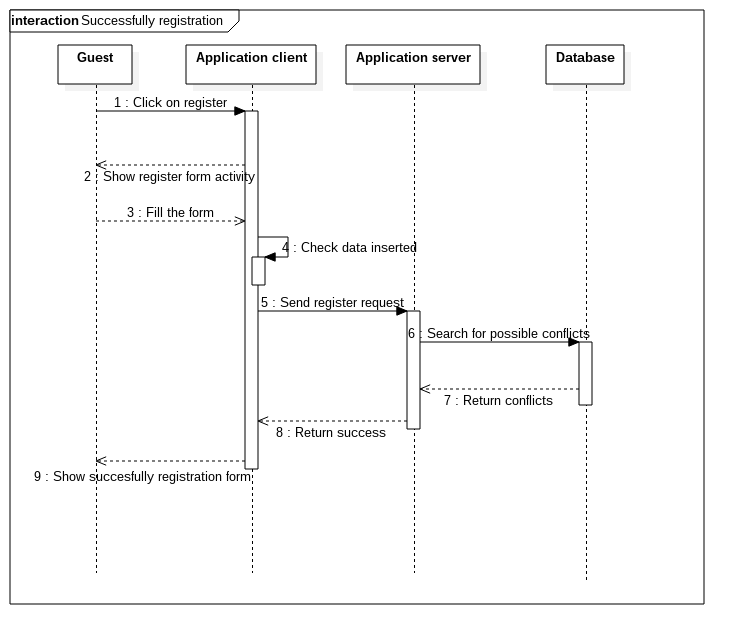
\includegraphics[scale=0.5]{Sequence Diagrams/successfully_registration.png}
\caption{ Registration }
\end{figure}
\newpage
\begin{figure} [h]
\centering
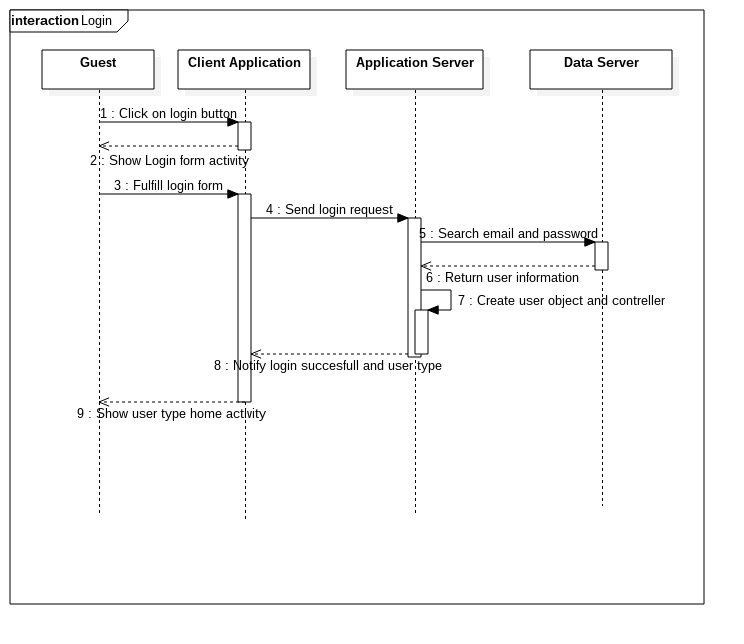
\includegraphics[scale=0.5]{Sequence Diagrams/login.png}
\caption{Login }
\end{figure}
\newpage
\begin{figure} [h]
\centering
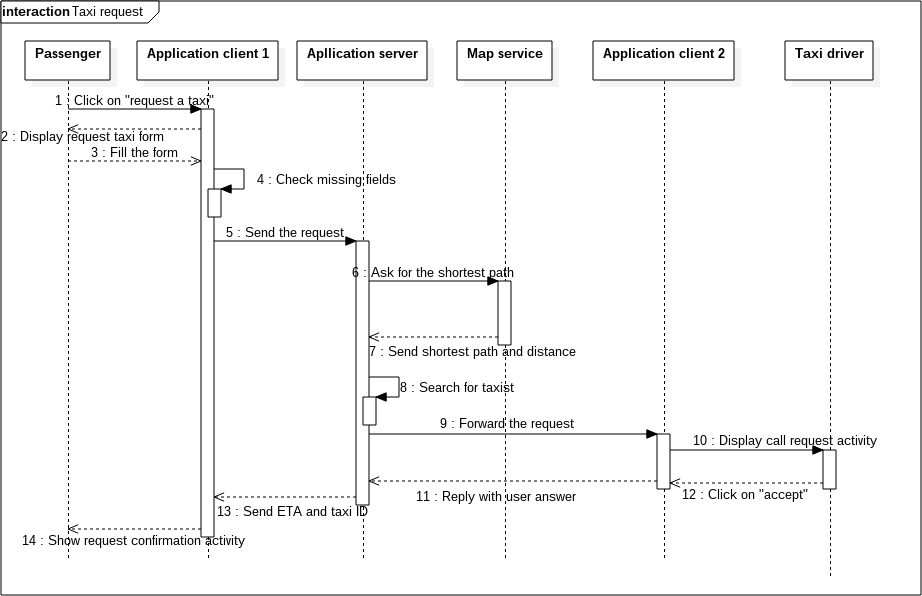
\includegraphics[scale=0.5]{Sequence Diagrams/successfully_taxi_request.png}
\caption{Taxi request }
\end{figure}
\newpage
\begin{figure} [h]
\centering
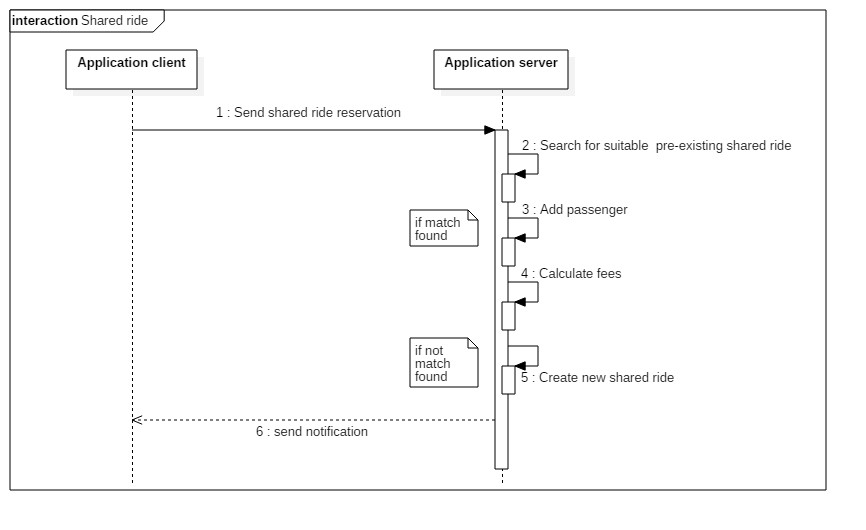
\includegraphics[scale=0.5]{Sequence Diagrams/Shared_ride.png}
\caption{Request of a shared ride }
\end{figure}
\newpage
\begin{figure} [h]
\centering
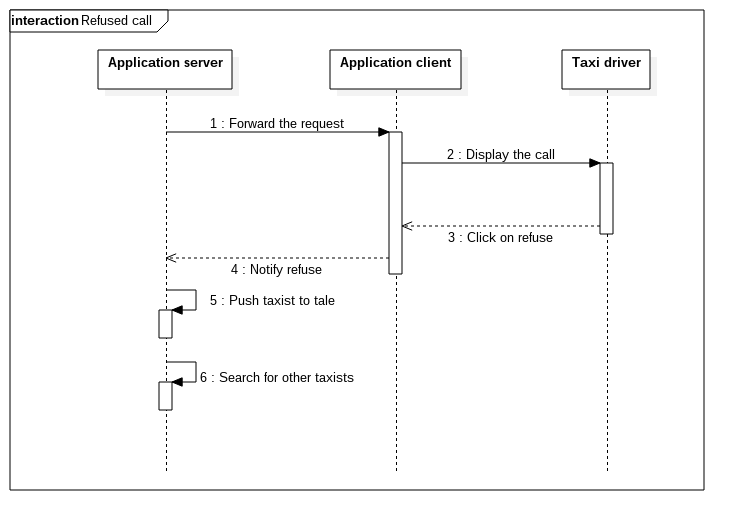
\includegraphics[scale=0.5]{Sequence Diagrams/refuse_call.png}
\caption{Refuse incoming call }
\end{figure}
\newpage
\begin{figure} [h]
\centering
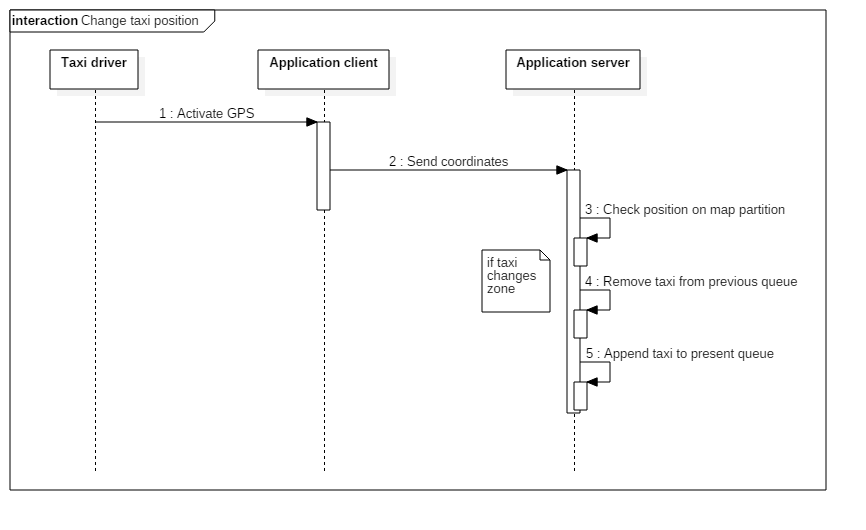
\includegraphics[scale=0.5]{Sequence Diagrams/change_taxi_position.png}
\caption{Change taxi position }
\end{figure}
\newpage
	\subsection{MVC diagrams}
\begin{figure} [h]
\centering
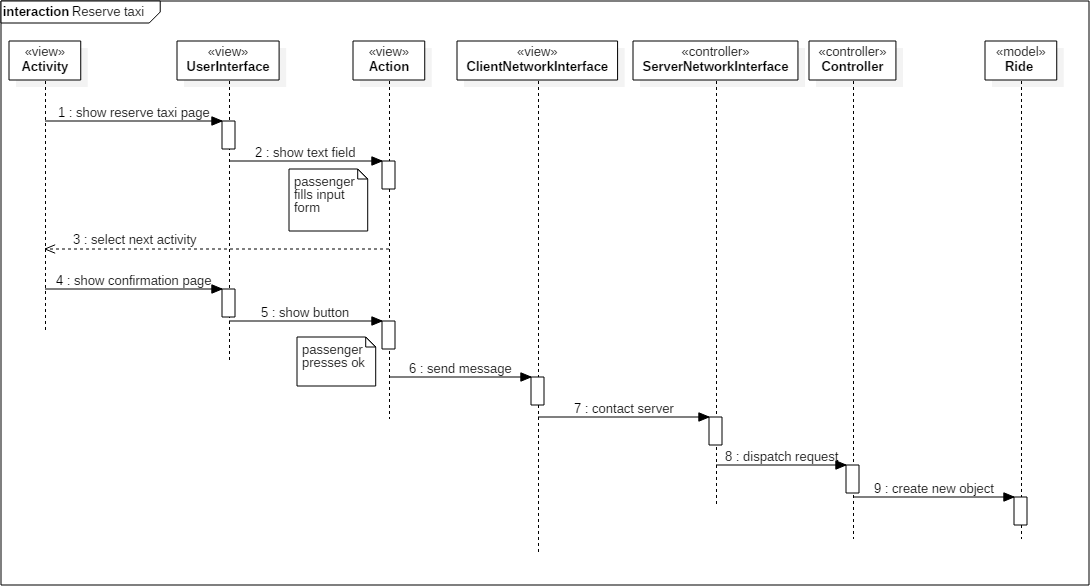
\includegraphics[scale=0.5]{Sequence Diagrams/MVC_reserve_taxi.png}
\caption{Reserve a taxi }
\end{figure}
\newpage
\begin{figure} [h]
\centering
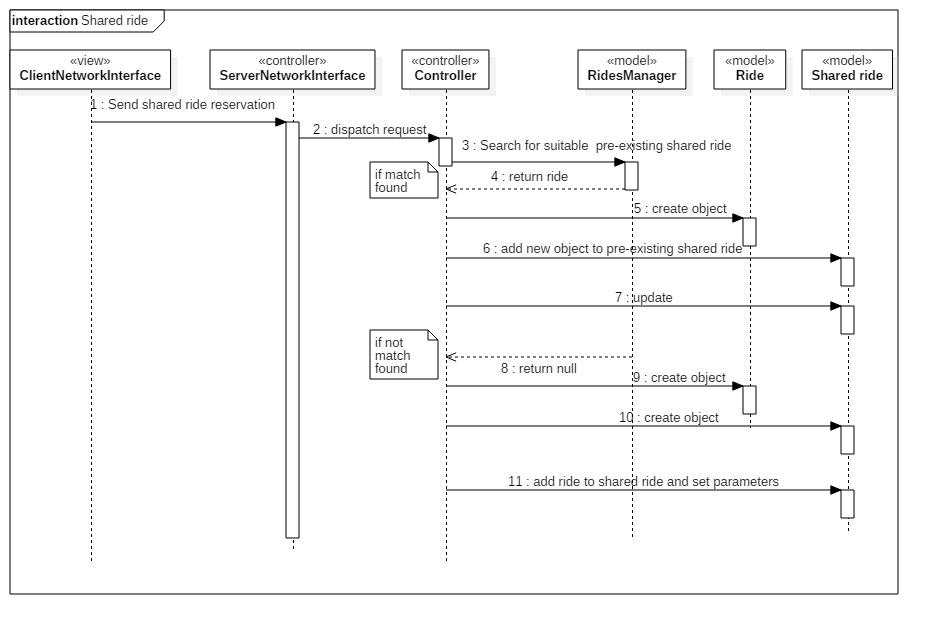
\includegraphics[scale=0.5]{Sequence Diagrams/MVC_Shared_ride.png}
\caption{Shared ride request }
\end{figure}
\newpage
%\hline %This was causing problems. I removed it, as I do for every problem blocking my righteous path
\newpage
\section{Component interfaces}

\subsection{Usage of third-party API}
The passenger controller class must interface with Google map sevice, using its API, to get the shortest path, the Eta to be sent to the user and the 
kilometers of the ride.

\subsection{In-house developed API}
The system must expose a set of public web based API. To access the API, an user must register first, using an unique key
obtained from the API's maintainer.
After successful registration, the system must return an authentication token to be used within a session.
The key and the token must be sent using the HTTP POST method; when needed, user-specific passwords must also
be sent via POST
The server will send the required data encoded in JSON form.
All the communications must be protected using the TLS protocol.
\begin{verbatim}
 https://api.mytaxiservice.com/registerapikey
\end{verbatim}
All the underlying functions (request taxis, list active calls, list taxis in a zone...) shall be made available using a simple,
object-like interface:
\begin{verbatim}
 https://api.mytaxiservice.com/request-ride/nonshared/<passengername>/
    <from_location>/<to_location>
 https://api.mytaxiservice.com/list-taxis/by-zone/<zone_id>
 https://api.mytaxiservice.com/list-calls/active/<passengername>/
 https://api.mytaxiservice.com/list-calls/active/<drivername>/
\end{verbatim}
A sample response (without the HTTP headers)
\begin{verbatim}
{
  type: "request_outcome",
  outcome: {
    taxi-id: "AZX934",
    eta: "12:30",
  }
}
\end{verbatim}

% socket?
% io (Il Vate(r)), suggerei di usare JSON per incapsulare i messaggi client-server, dato chè è il metodo più
% semplice e anche popolare per questi usi
\section{Selected architectural styles and patterns}
The application follows the MVC (Model-View-Controller) pattern.
The model is entirely contained in the server side, and it's composed by a singleton class (Ridesmanager), that contains 
informations shared by all the controllers, and a user class (User), that contains informations about a specific user, and is
accessible only by the controller assigned to the corresponding user.
Furthermore, the view is completely contained in the client side; it is composed by the ``userinterface'' class, that must display
the activity's objects.
The controller is mainly represented by the homonym class, in the server side. There are few controller's functions , that don't 
require data contained in the server, implemented in the action class.

\section{Other design decisions}
The server side structure is composed as shown in Figure \ref{fig:hwarch}:
The load balancer is needed to equally divides requests coming from different clients, in order to increase performances.
%Different application servers must be placed in different physical zones, in order to react to possibly partial blackout and other
%local physical accidents.
For the client side there's only one constraint, the obligation for the taxi driver to use a device with a working GPS.

\begin{figure} [h]
  \centering
  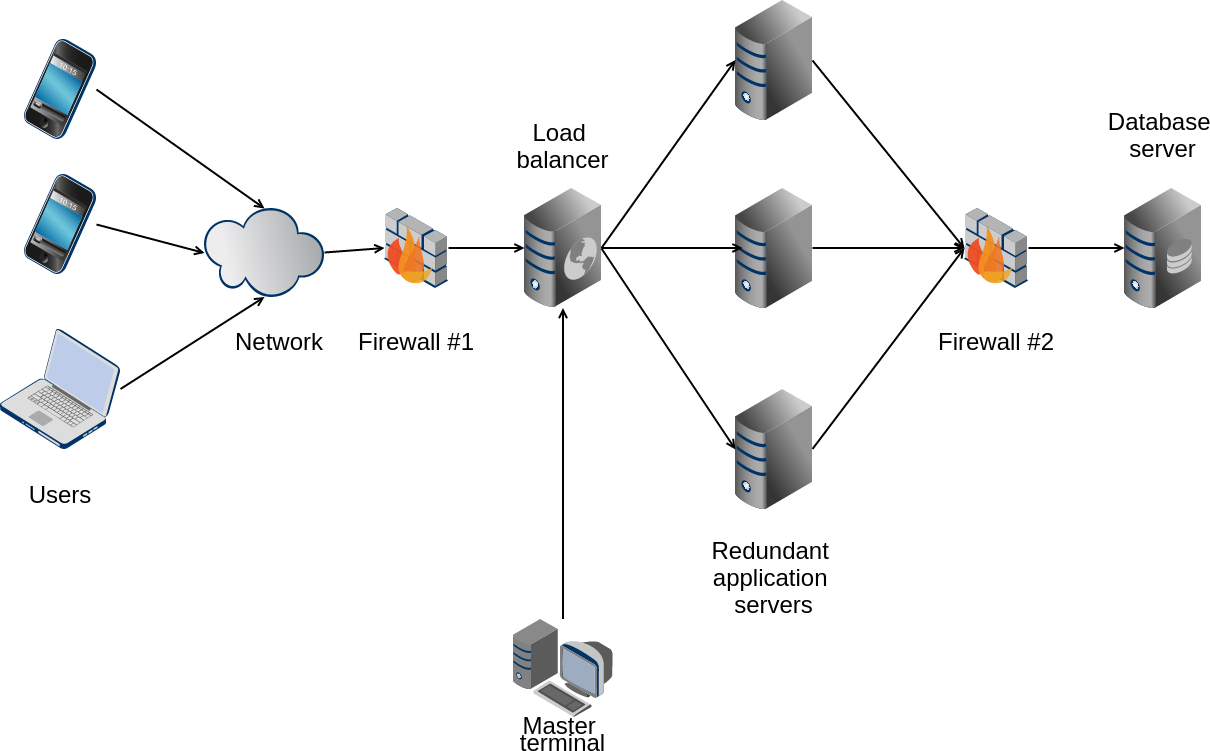
\includegraphics[scale=0.35]{../../architecture/architecture.png}
\caption{Server architecture \label{fig:hwarch}}
\end{figure}
